\documentclass[11pt]{report}
\title{Computer Networks - RCp}
\author{Nuno Brito}
%\date{}

%packaging
\usepackage{graphicx}                                   % Inserir imagens
    \graphicspath{ {./images/} }                        % Caminho para o recurso imagens
\usepackage[portuguese]{babel}                          % Pacote que descarrega e traduz linguagem global dos campos pré-definidos de LaTeX
    \selectlanguage{portuguese}                         % Define linguagem para português
\usepackage{multicol}                                   % Criar texto em colunas (\begin{multicols}{#} [...] \end{multicols}). Usar \raggedcolumns e \columnbreak
    \setlength{\columnsep}{3cm}                         % Define espaçamento entre múltiplas colunas
\usepackage{longtable}
\usepackage{listings}                                   % Para código
%\usepackage{comment}                                    % Permite criar um segmento de comentários (/begin{comment} [...] /end{comment})
%\usepackage{xcolor}                                     % Colorir texto (esta versão é mais flexível do que a {color})
%\usepackage{subcaption}                                 % Subcaptions para figuras
%\usepackage{fullpage}                                   % Utilizar página inteira
    \lstdefinestyle{pythoncode}
    {
        %backgroundcolor=\color{backcolour},
        %commentstyle=\color{codegreen},
        %keywordstyle=\color{magenta},
        %numberstyle=\tiny\color{codegray},
        %stringstyle=\color{codepurple},
        %basicstyle=\ttfamily\footnotesize,
        breakatwhitespace=false,
        breaklines=true,
        captionpos=b,
        keepspaces=true,
        numbers=left,
        numbersep=5pt,
        showspaces=false,
        showstringspaces=false,
        showtabs=false,
        tabsize=2
        %inputencoding=utf8,
        %extendedchars=true,
    }

\begin{document}

\tableofcontents

\section{Introduction}
    Milestones:
    \begin{itemize}
        \item Getting apache2 web server running in localhost
        \item Access web server - http://127.0.0.1/
        \item Access web server from other computer
        \item Use wireshark to capture the web access from another host
        \item Compare the HTTP headers sent by the client and the server
        \item Develop a web client
        \item Establish a TCP connection to the server
        \item Request the base webpage
    \end{itemize}
    
    Web client requirements:
    \begin{itemize}
        \item Usage of HTTP library forbidden
        \item Establish TCP connection using available sockets library - send the HTTP request and receive the HTTP reply
        \item HTTP reply should be presented to the user
        \item - Optional - act to the various HTTP replies
        \item Text-only application
    \end{itemize}

\section{Project}
    \subsection{Software}
        local server:
            windows 11 x64
            xampp-portable-windows-x64-8.2.12-0-VS16.7z
        client:
            firefox version
            librefox version
            wireshark version
    
    \subsection{Configurations}
        SSLEngine disabled in apache to ease access with http
        %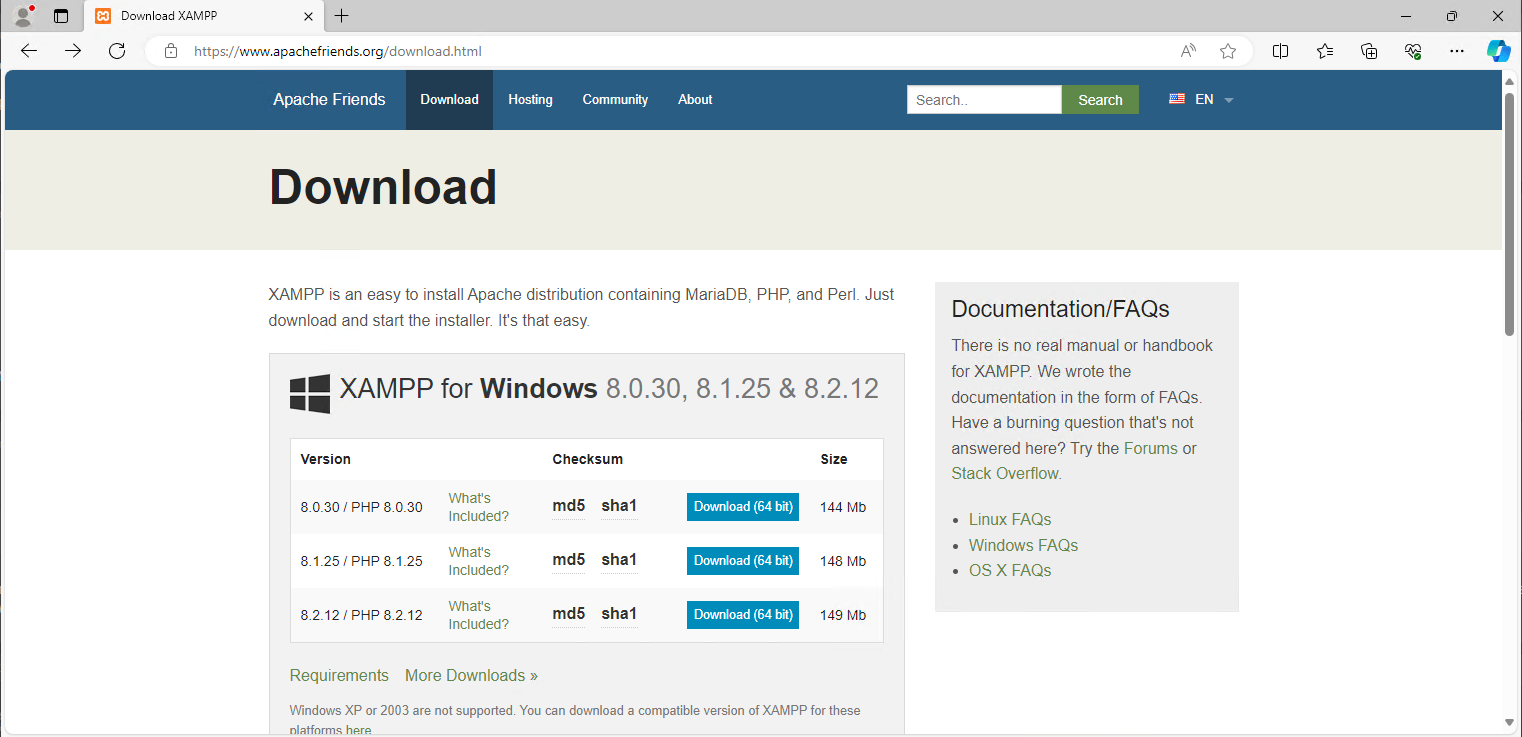
\includegraphics[scale=1.0]{xampp01} \\
        %<=++figure sslengine off++=>
        %<=++figure access from localhost++=>
        %<=++figure access from 127.0.0.1++=>
        %<=++figure access from anotherhost++=>
        %<=++figure wireshark capture from another host++=>
    
    \subsection{Python code}
        \lstset{style=pythoncode}
        \lstinputlisting[language=python, caption=Simple HTTP webclient using sockets in python]{webclient/httpsocketv3.py}
        The code was adapted to be simple and cycle through the various responses.
        Modifiable variables include serverName, serverPort and the httpTestMessages list.
        The httpTestMessages is built in a way that only the first part is necessary to modify.
    
    \subsection{List of headers}
        client
            meaning
        server
            meaning
    
    \subsection{Objectives}
        Step-by-step instructions performed
        Xampp install
        wireshark install
        wireshark settings
        wireshark filters
        
        \begin{tabular}{ l r }
            text & 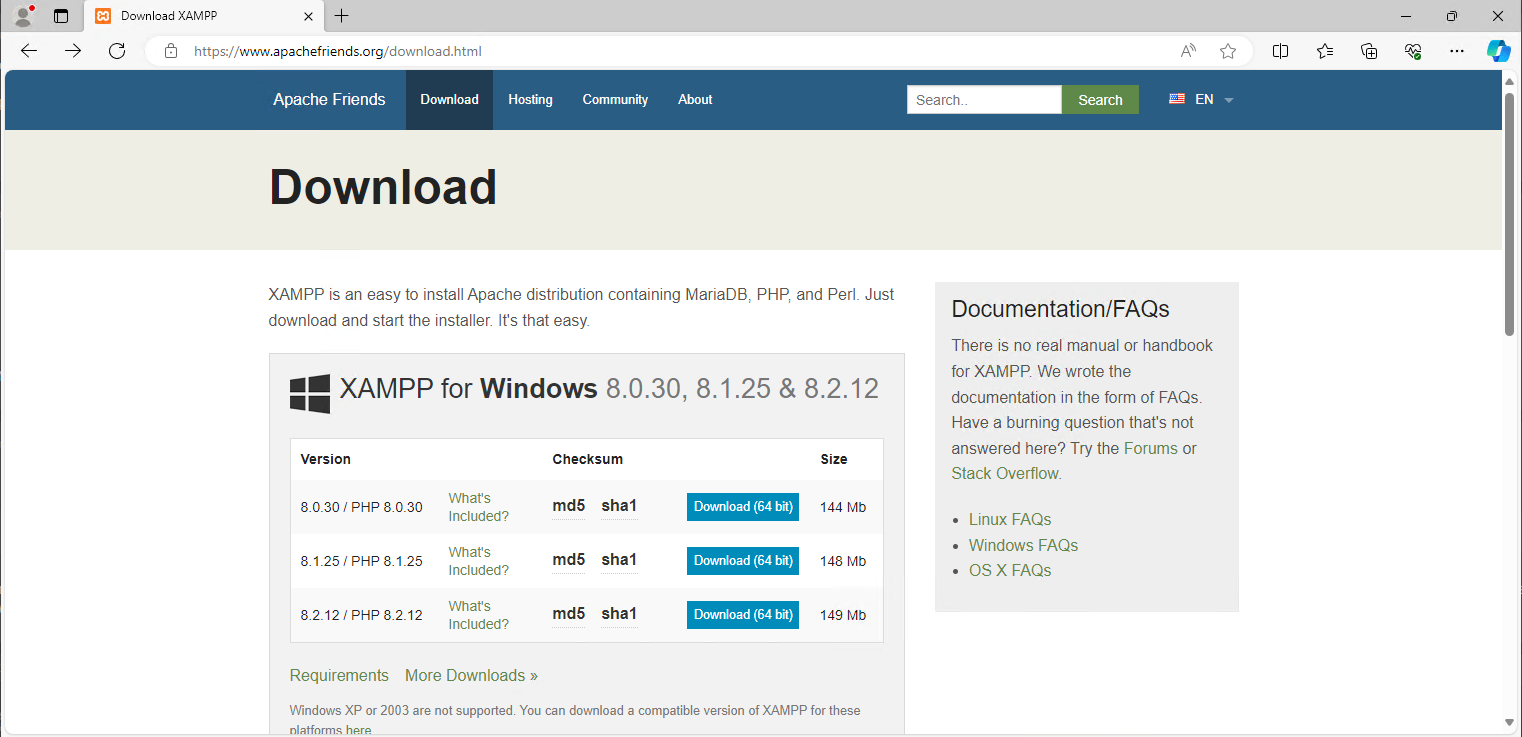
\includegraphics[scale=1.0]{xampp01} \\ % 0.3 scale!
            text & 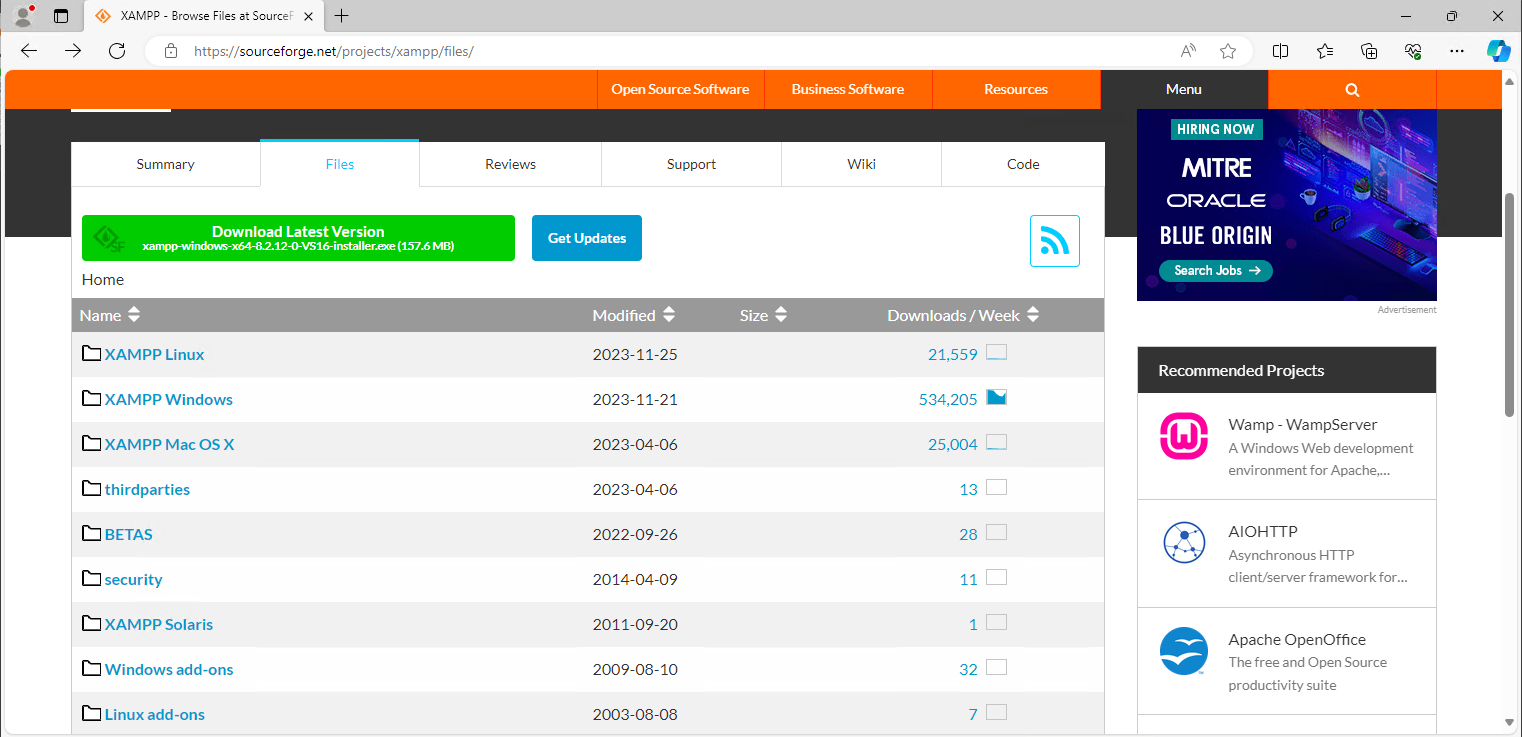
\includegraphics[scale=1.0]{xampp02} \\
            text & 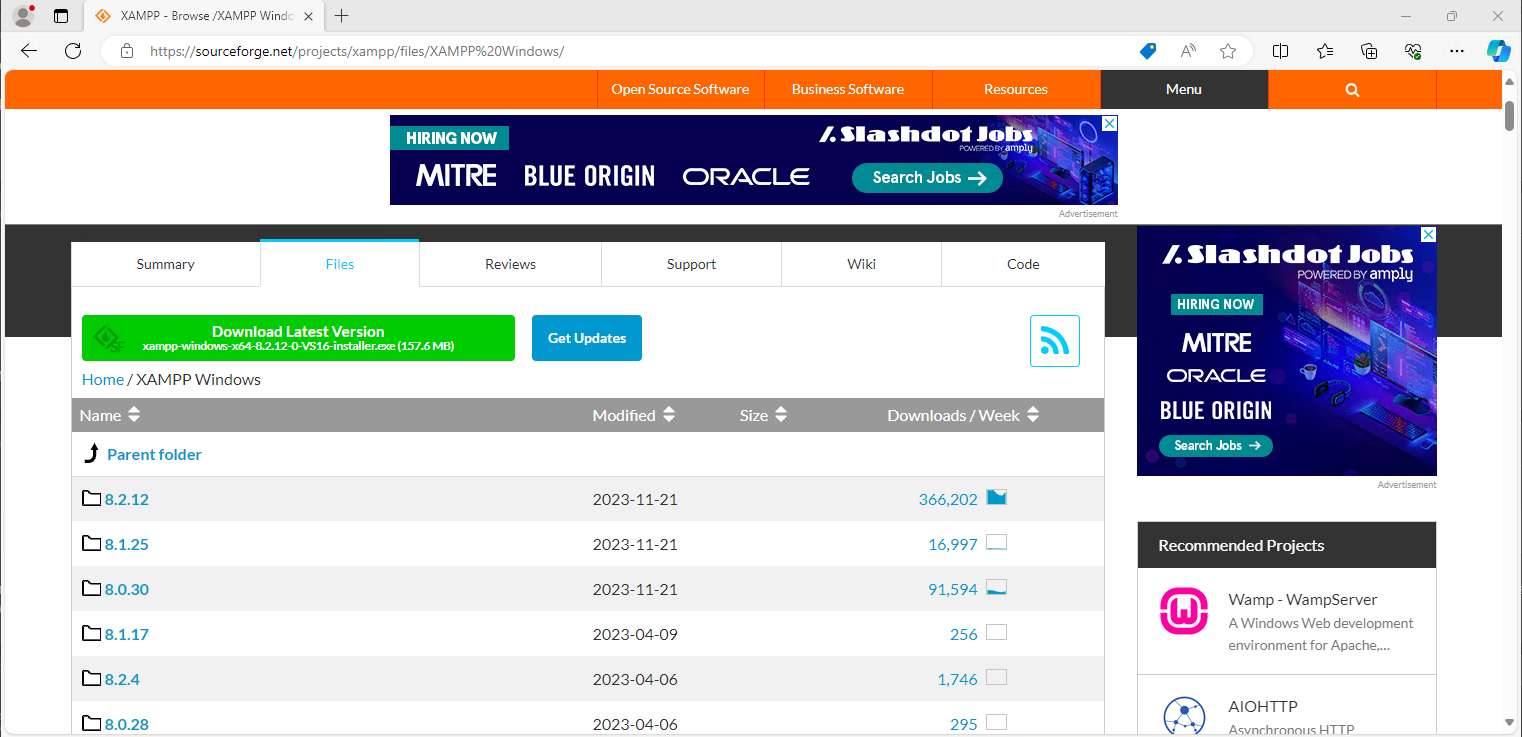
\includegraphics[scale=1.0]{xampp03} \\
            text & 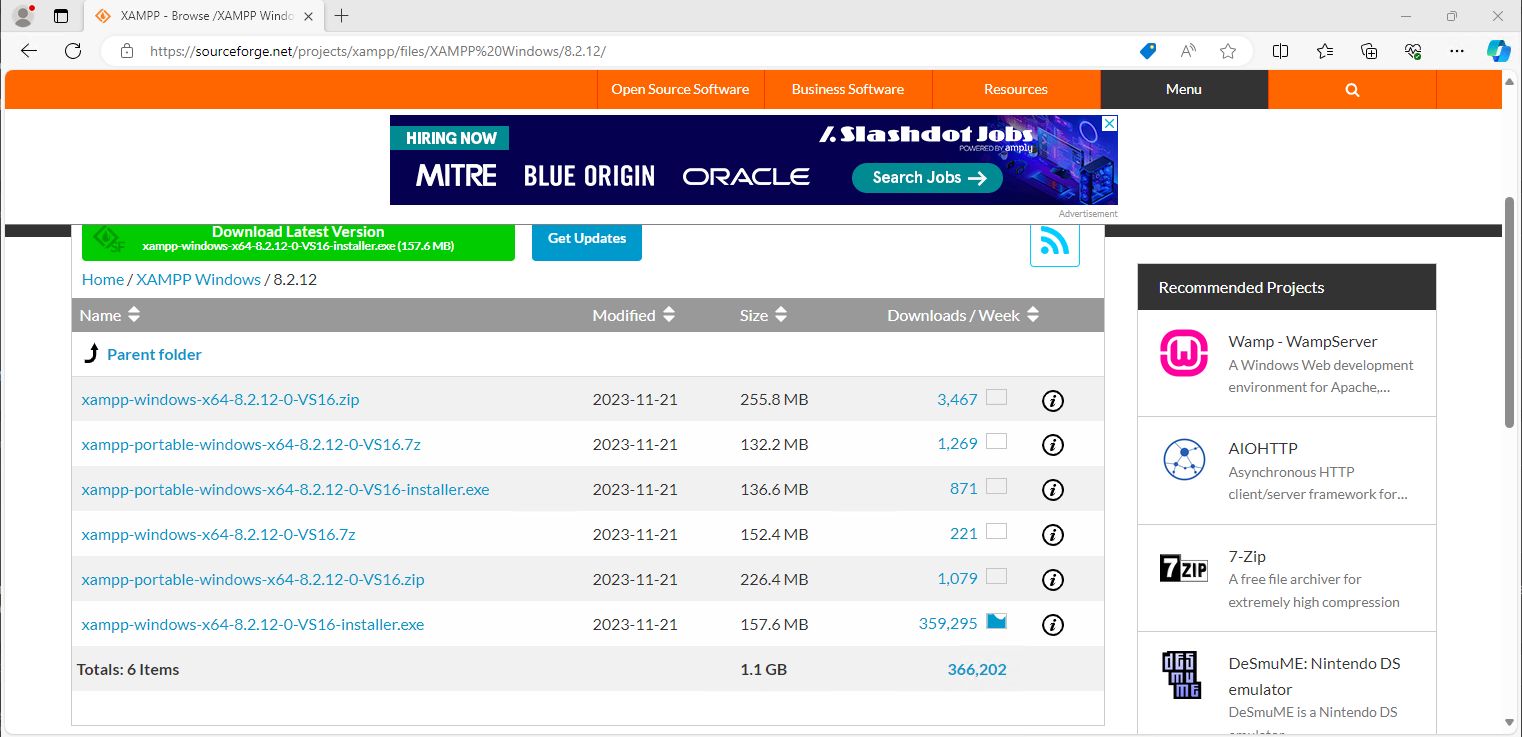
\includegraphics[scale=1.0]{xampp04} \\
            text & 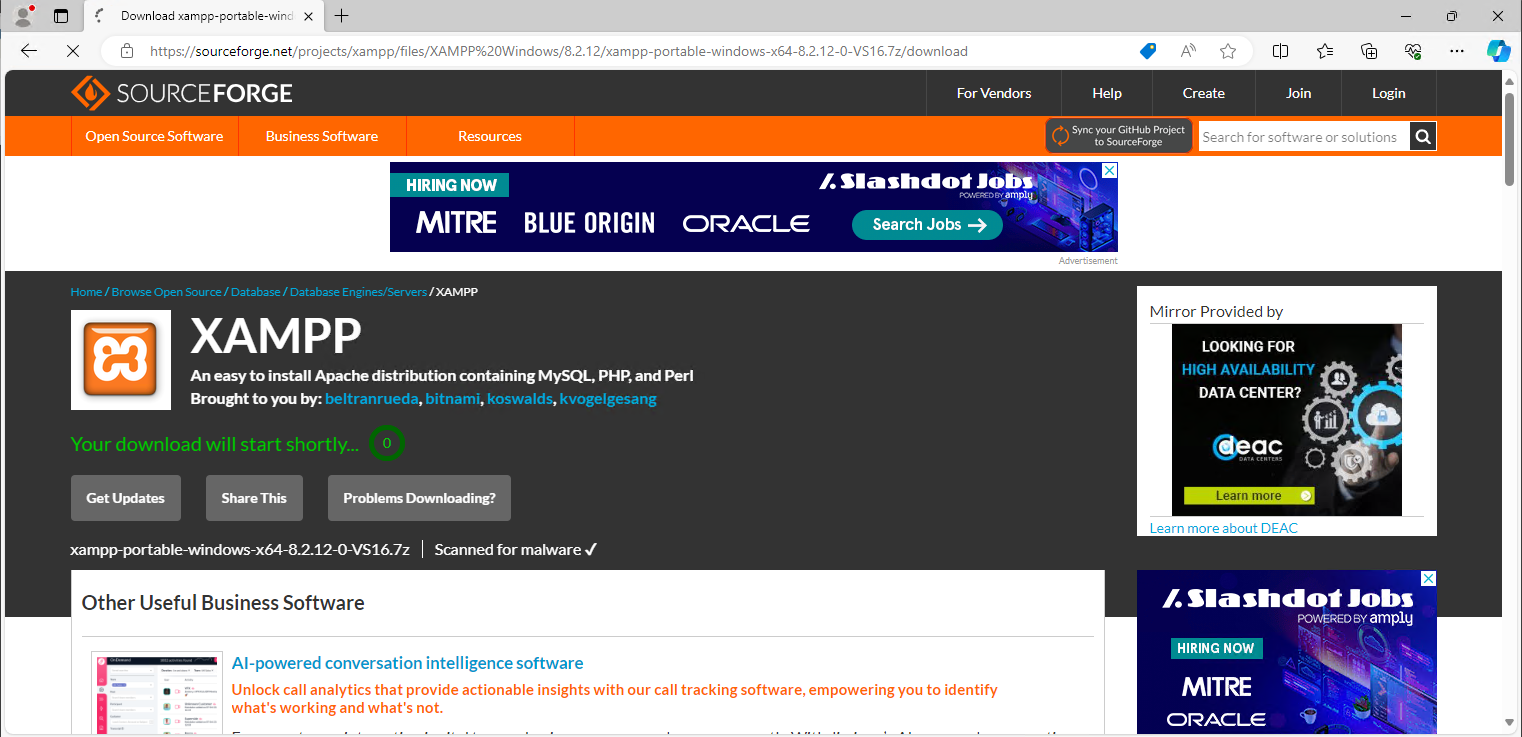
\includegraphics[scale=1.0]{xampp05} \\
            text & 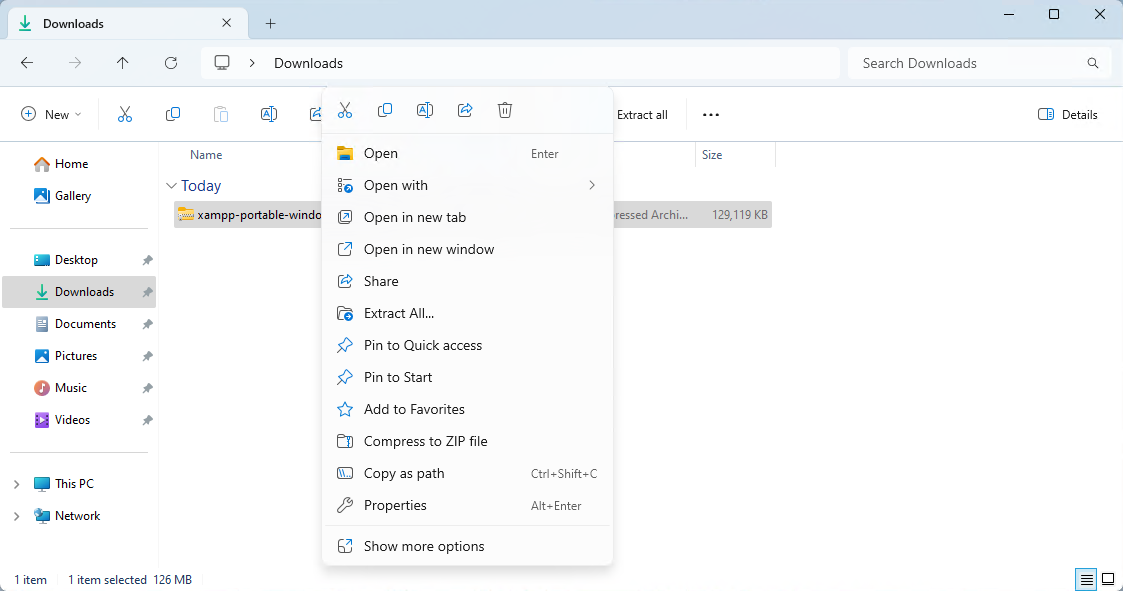
\includegraphics[scale=1.0]{xampp06} \\
            text & 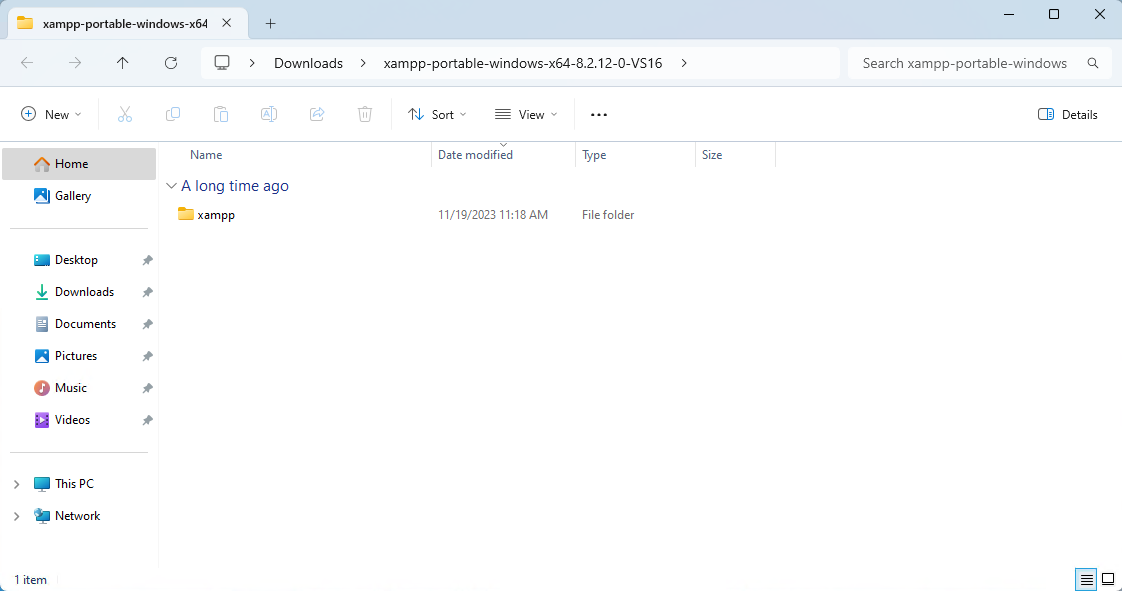
\includegraphics[scale=1.0]{xampp07} \\
            text & 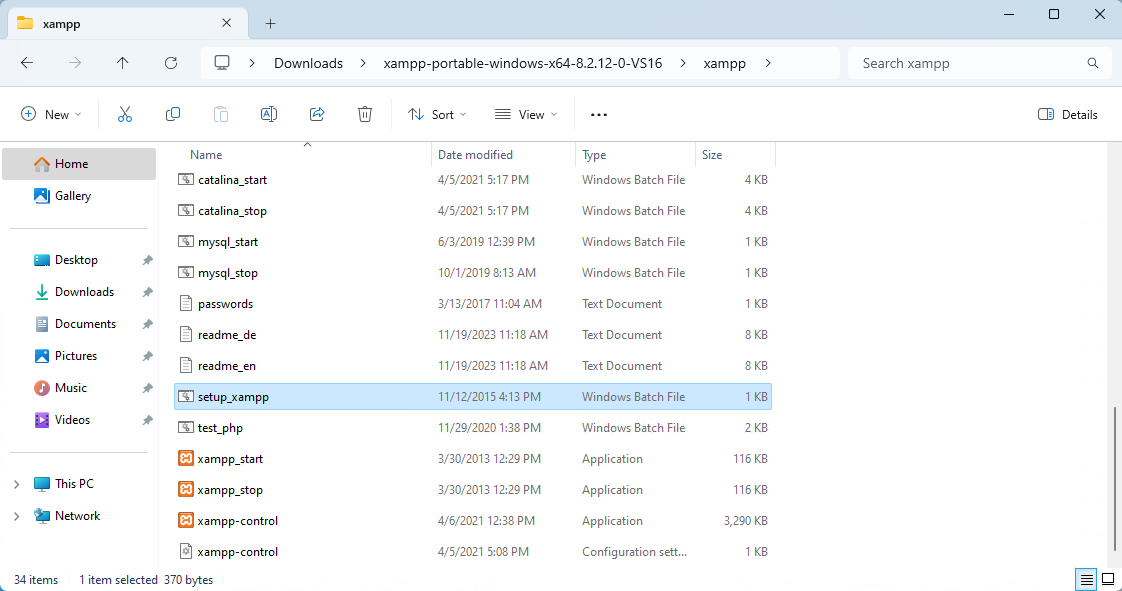
\includegraphics[scale=1.0]{xampp08} \\
            text & 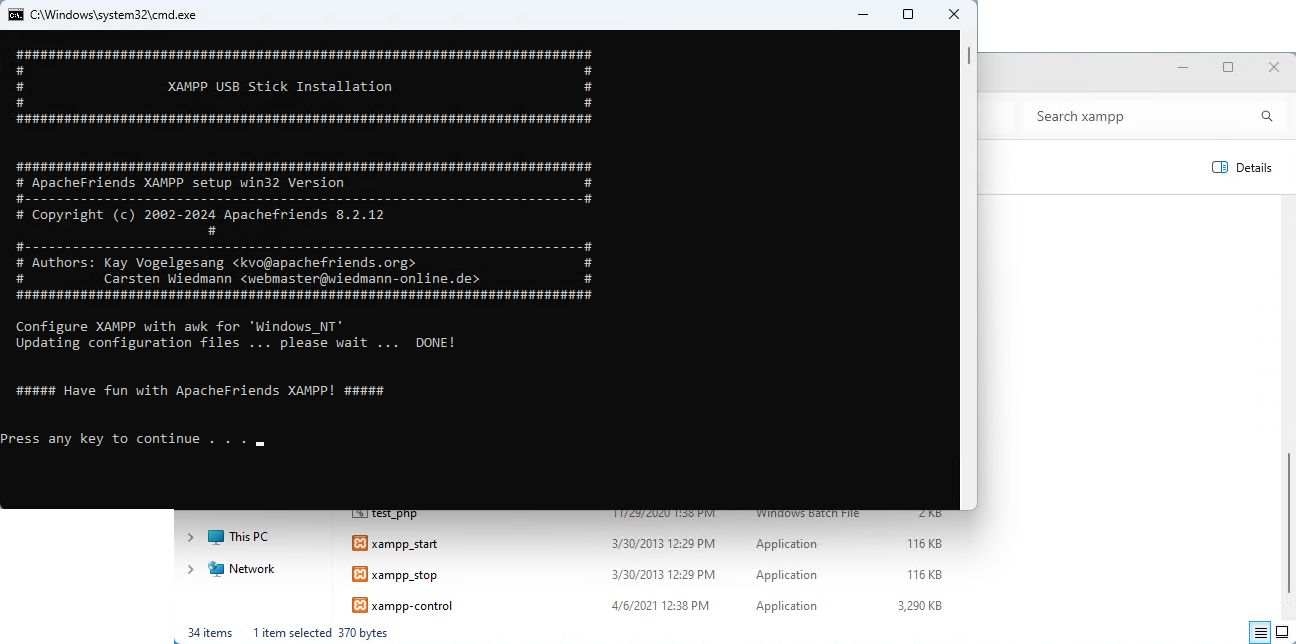
\includegraphics[scale=1.0]{xampp09} \\
            text & 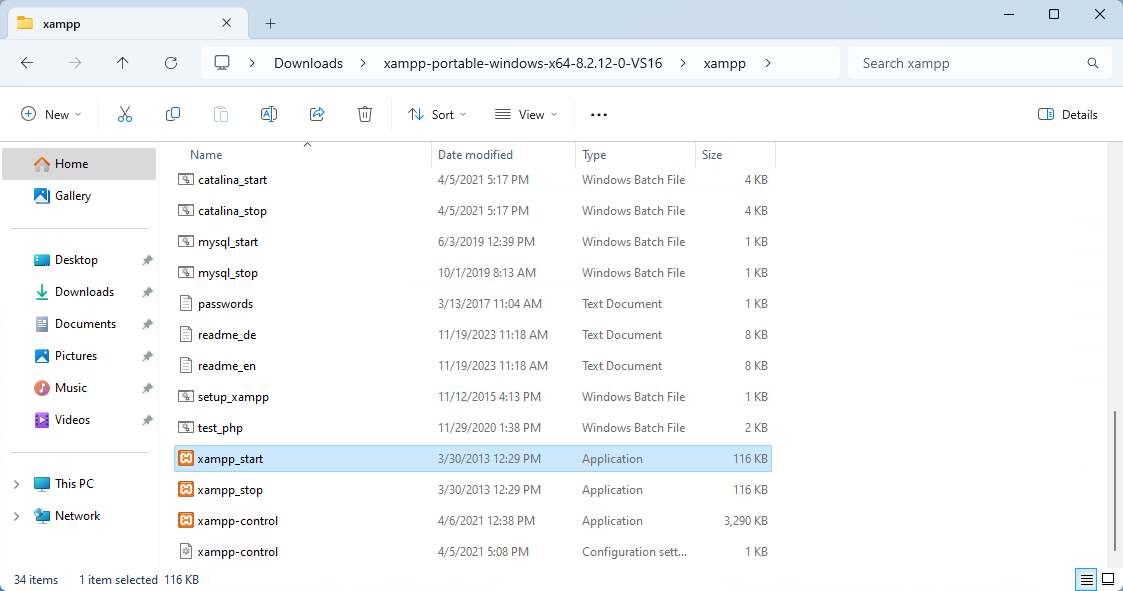
\includegraphics[scale=1.0]{xampp10} \\
            text & 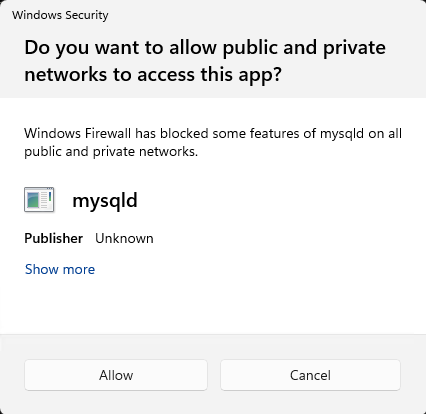
\includegraphics[scale=1.0]{xampp11} \\
            text & 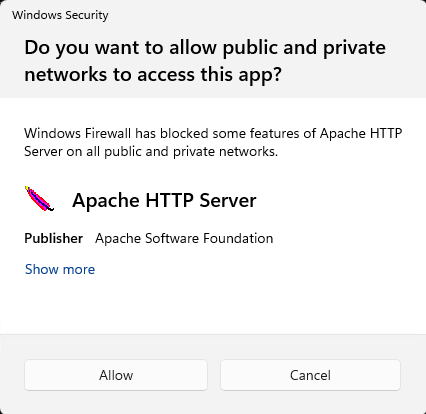
\includegraphics[scale=1.0]{xampp12} \\
            text & 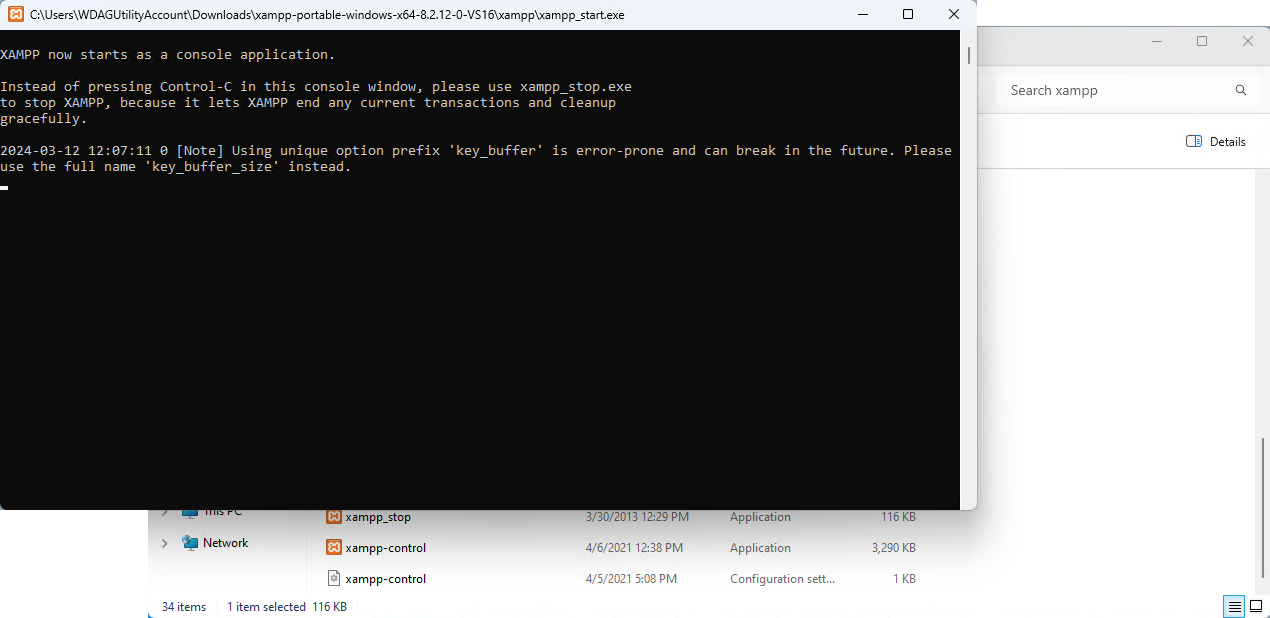
\includegraphics[scale=1.0]{xampp13} \\
            text & 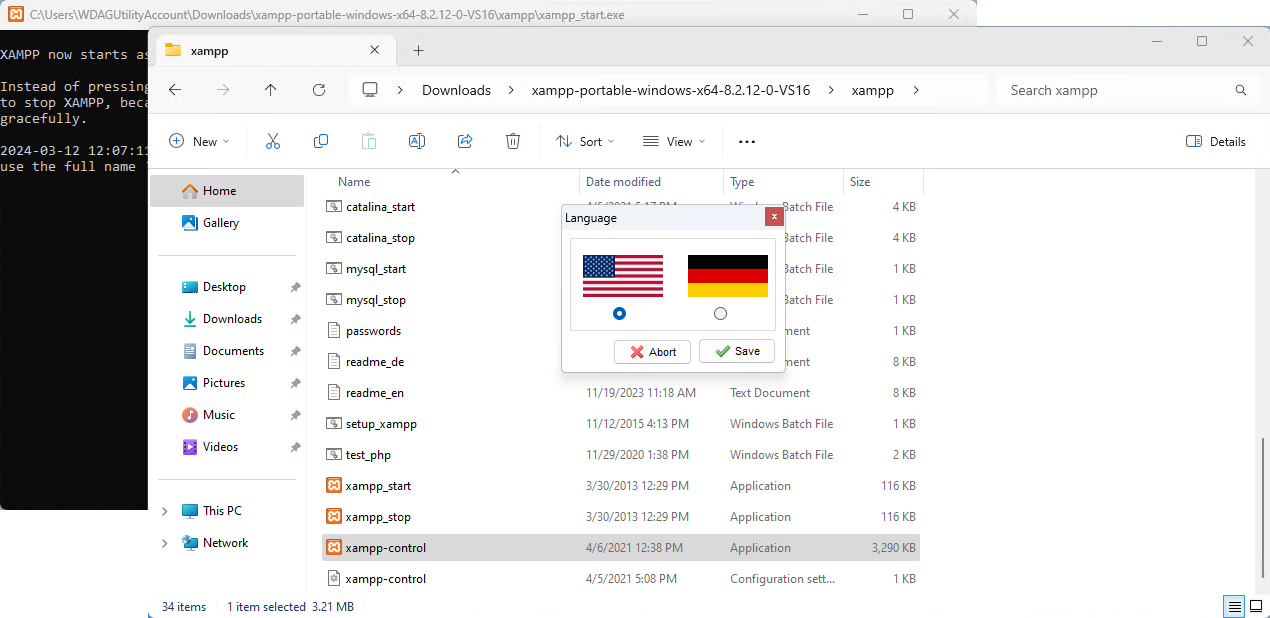
\includegraphics[scale=1.0]{xampp14} \\
            text & 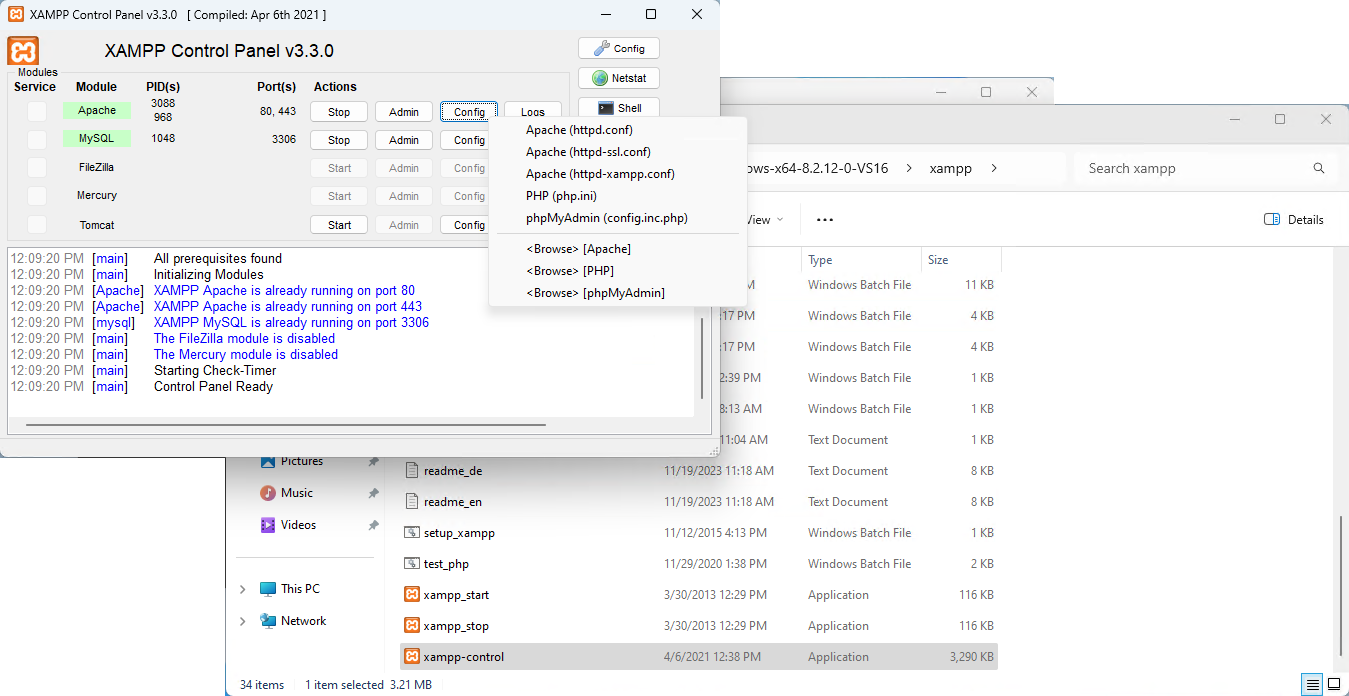
\includegraphics[scale=1.0]{xampp15} \\
            text & 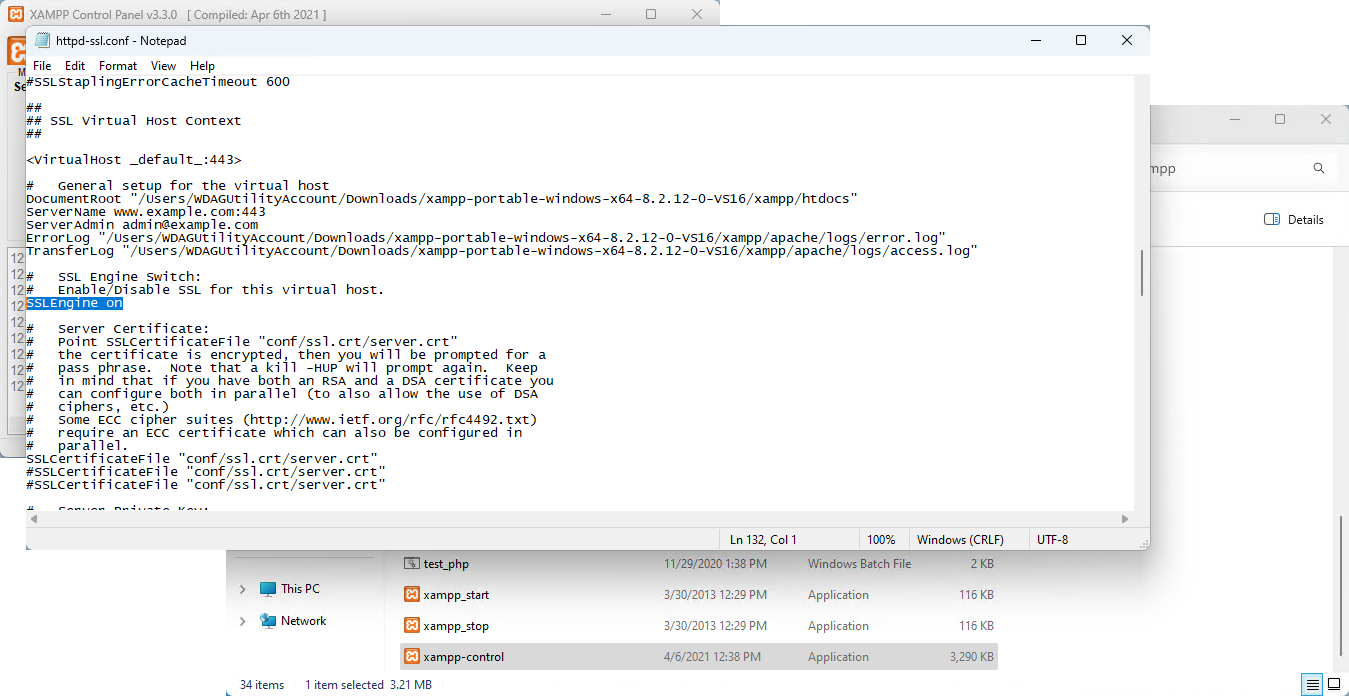
\includegraphics[scale=1.0]{xampp16} \\
            text & 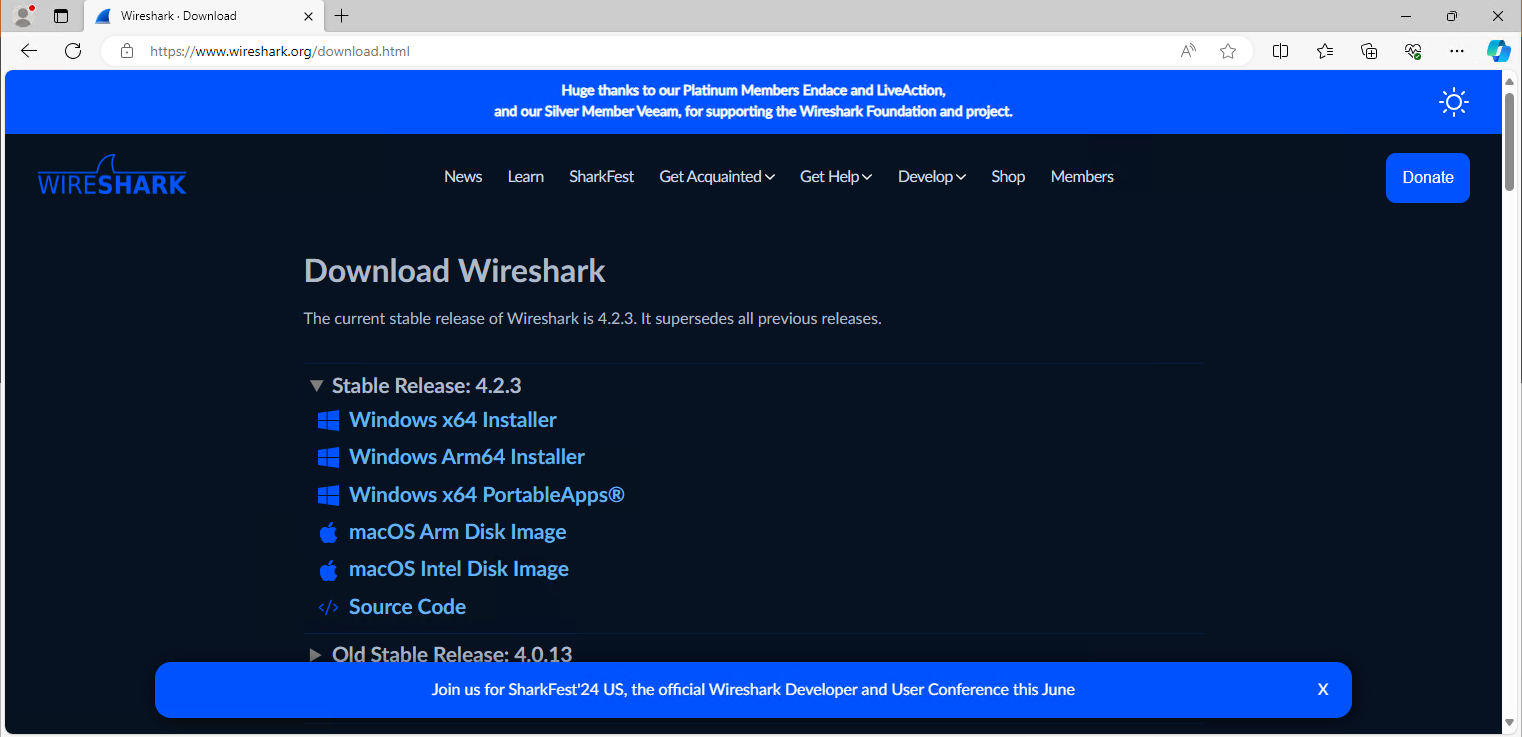
\includegraphics[scale=1.0]{wireshark01} \\
            text & 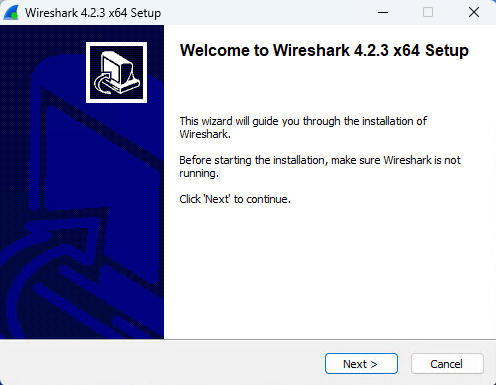
\includegraphics[scale=1.0]{wireshark02} \\
            text & 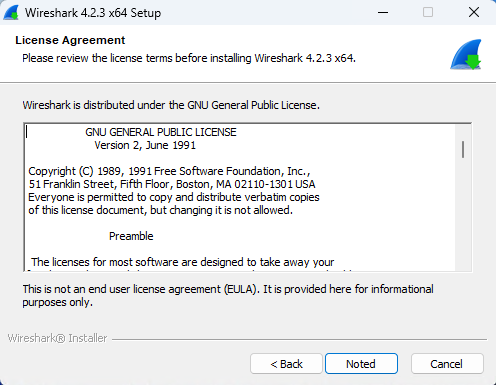
\includegraphics[scale=1.0]{wireshark03} \\
            text & 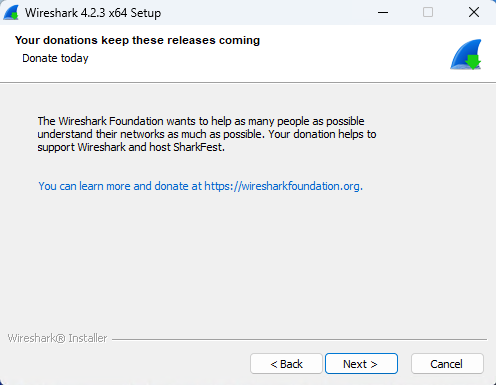
\includegraphics[scale=1.0]{wireshark04} \\
            text & 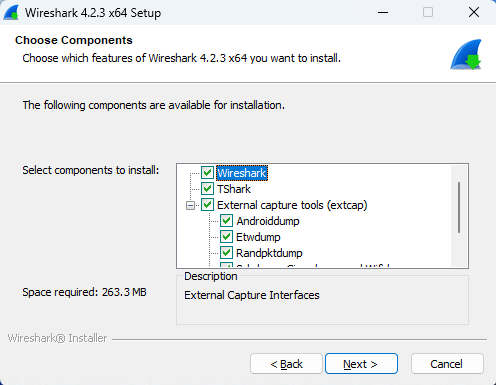
\includegraphics[scale=1.0]{wireshark05} \\
            text & 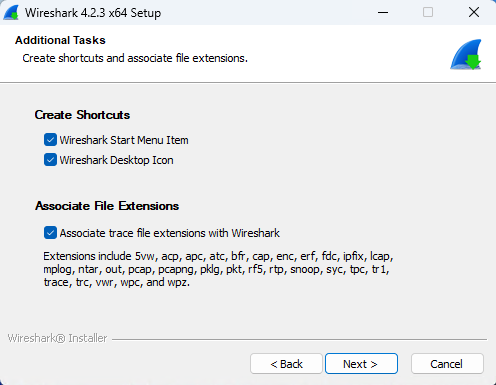
\includegraphics[scale=1.0]{wireshark06} \\
            text & 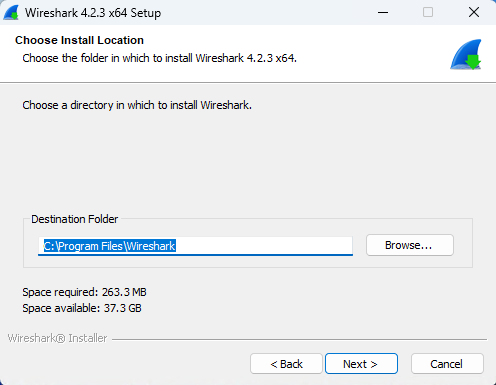
\includegraphics[scale=1.0]{wireshark07} \\
            text & 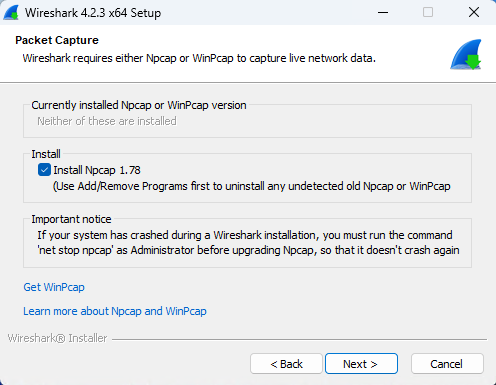
\includegraphics[scale=1.0]{wireshark08} \\
            text & 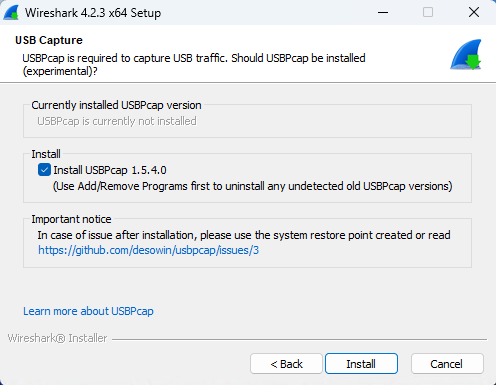
\includegraphics[scale=1.0]{wireshark09} \\
            text & 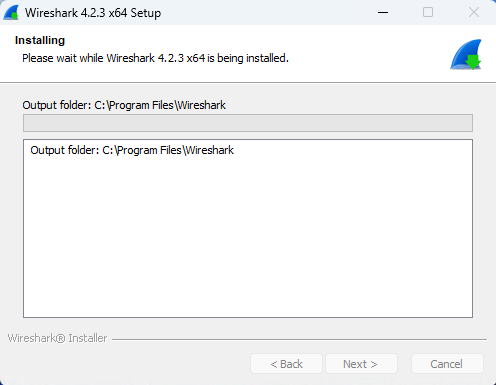
\includegraphics[scale=1.0]{wireshark10} \\
            text & 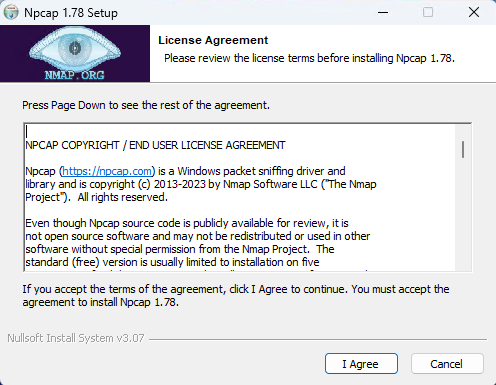
\includegraphics[scale=1.0]{wireshark11} \\
            text & 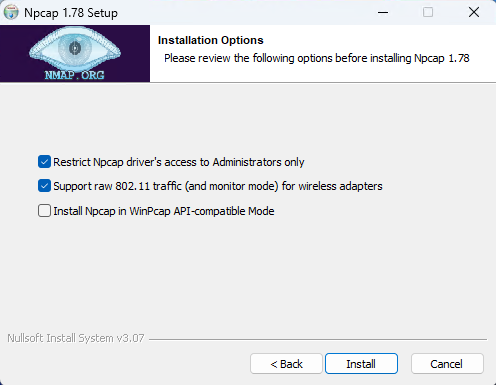
\includegraphics[scale=1.0]{wireshark12} \\
            text & 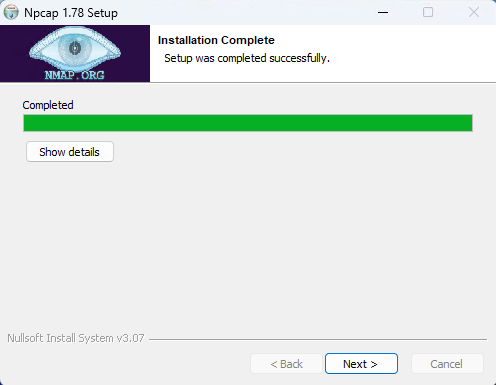
\includegraphics[scale=1.0]{wireshark13} \\
            text & 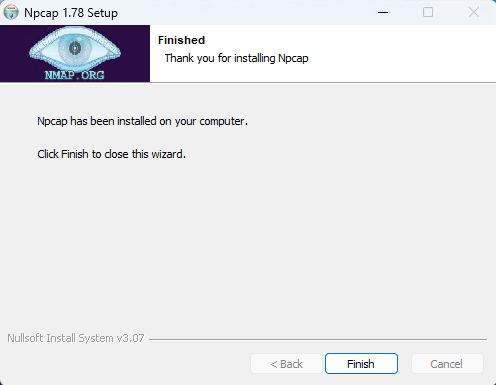
\includegraphics[scale=1.0]{wireshark14} \\
            text & 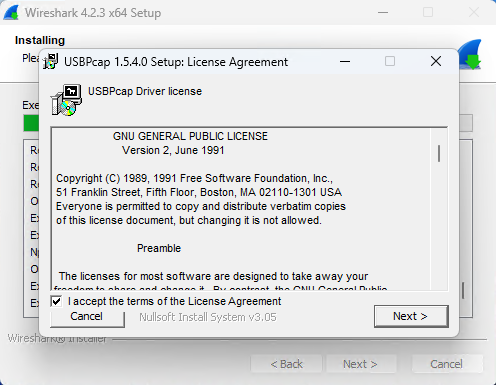
\includegraphics[scale=1.0]{wireshark15} \\
            text & 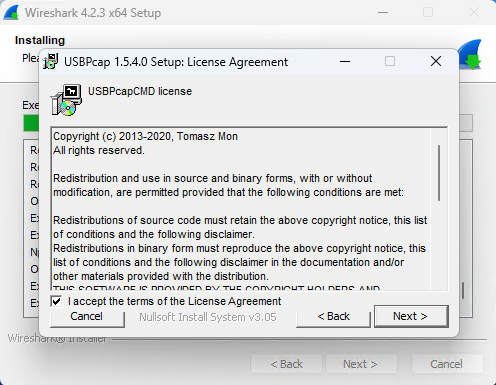
\includegraphics[scale=1.0]{wireshark16} \\
            text & 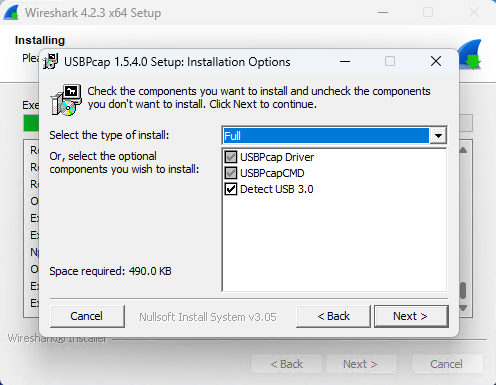
\includegraphics[scale=1.0]{wireshark17} \\
            text & 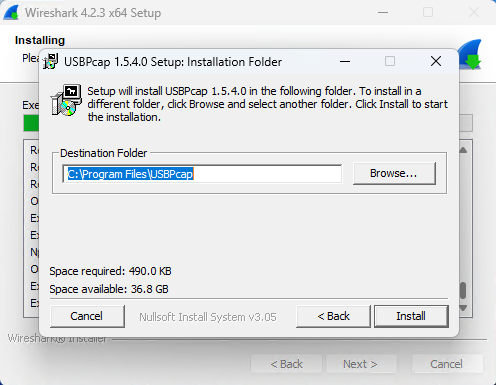
\includegraphics[scale=1.0]{wireshark18} \\
            text & 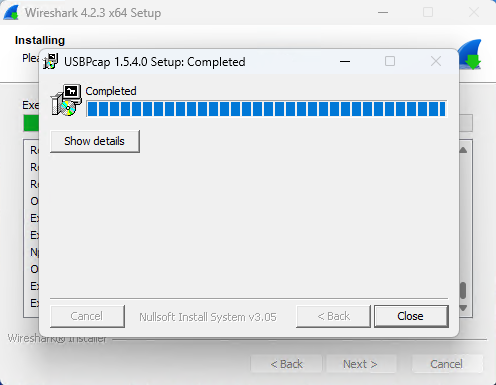
\includegraphics[scale=1.0]{wireshark19} \\
            text & 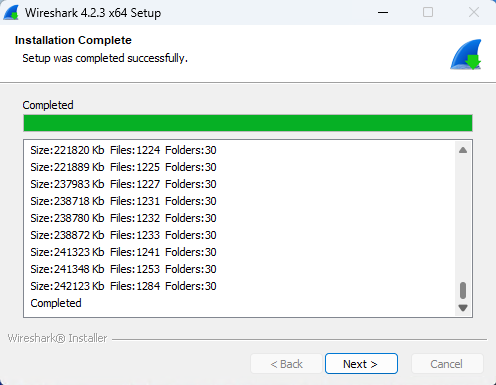
\includegraphics[scale=1.0]{wireshark20} \\
            text & 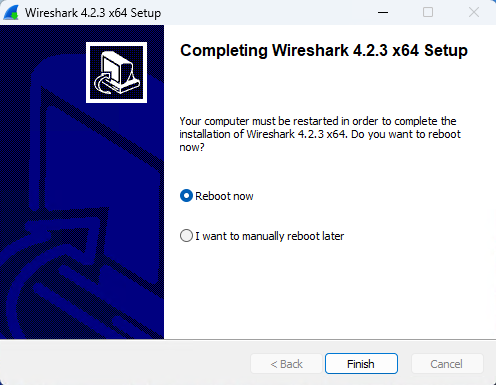
\includegraphics[scale=1.0]{wireshark21} \\
        \end{tabular}
        
        \begin{multicols}{2}
        [Install]
        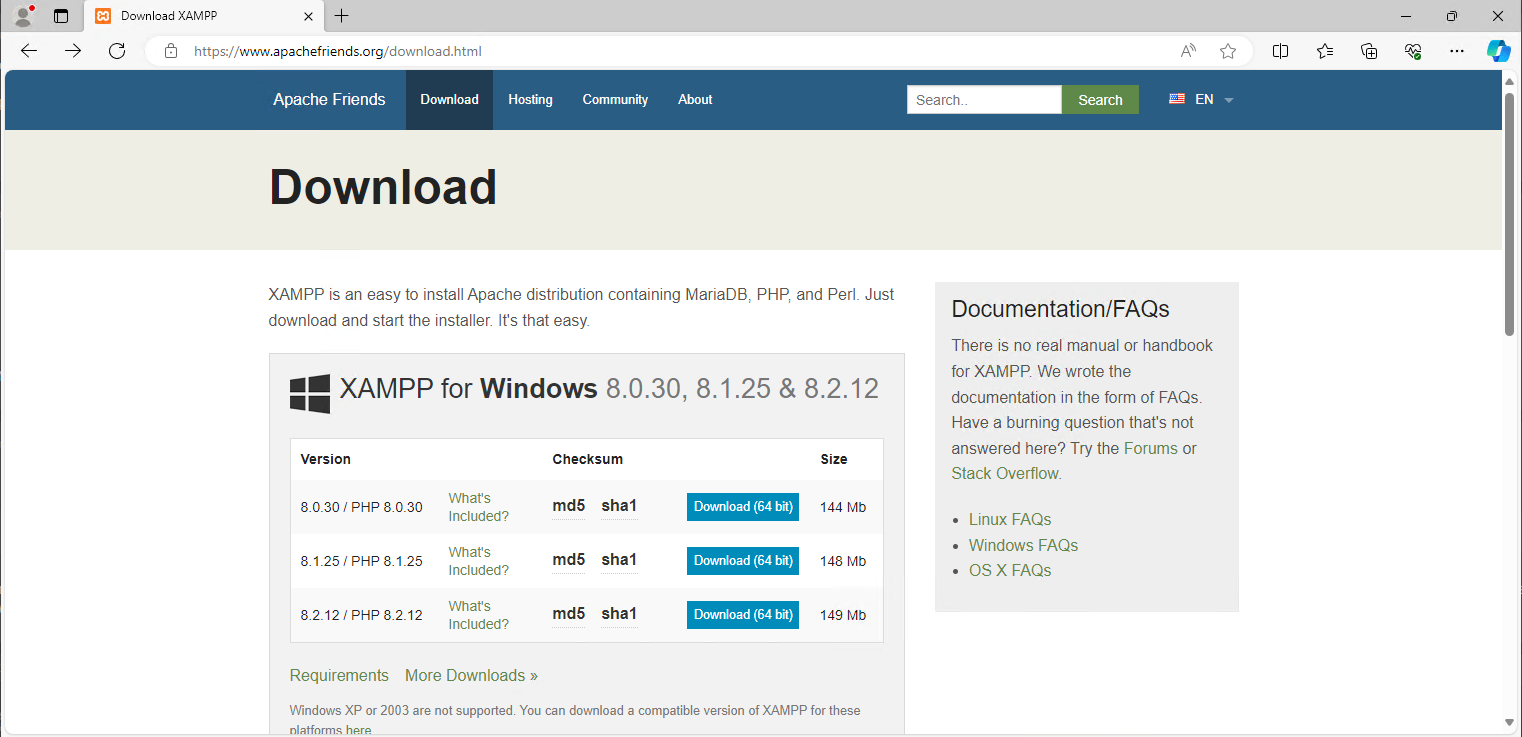
\includegraphics[scale=1.0]{1}

\section{Problems and resolutions}
    Python code: default system came with python2. Python3 installed.
    Encrypted html body: since the xampp server is running in a laptop at home and to make some progress i have to work remotely via vpn, the content came encrypted.
    Default http protocol SSL: disabled in apache2 the ssl engine

\end{document}
